\documentclass[12pt]{beamer}
\usepackage{natbib}
\usepackage[francais]{babel}
\usepackage[T1]{fontenc}
\usepackage[utf8]{inputenc}
\usepackage{amsmath}
\usepackage{amsfonts}
\usepackage{lmodern}
\setbeamercovered{transparent=20}

\usepackage{graphicx}

\usetheme{CambridgeUS}

\title{Introduction to Process Virtual Memory}
\author{Stanislas Plessia}
\date{2016}


\begin{document}
	
\begin{frame}
	\titlepage
\end{frame}


\begin{frame}{How does it look like ?}
	\begin{figure}[h!]
		\centering
		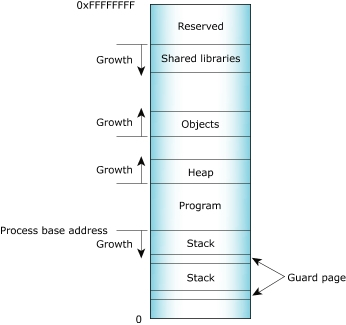
\includegraphics[width=5cm]{1.jpg}
		\caption{Process Memory}
	\end{figure}
\end{frame}

\begin{frame}{How is the physical/virtual Mapping done}
	\begin{figure}[h!]
		\centering
		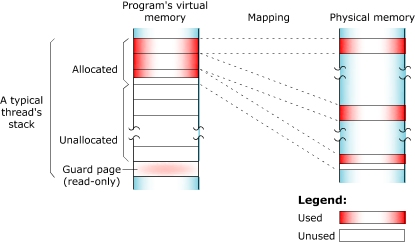
\includegraphics[width=9cm]{4.jpg}
		\caption{Physical Mapping}
	\end{figure}
\end{frame}

\begin{frame}{What it's used for}
	\begin{itemize}
		\item<1-> Program : \uncover<2>{Contains the executable content of the program (code + data)}
		\item<3-> Stack : \uncover<4>{Contains all the local variables and parameters needed for the program to run}
		\item<5-> Libraries : \uncover<6>{Shared Libraries like libc}
		\item<7-> Objects : \uncover<8>{To map hardware components memory into the process memory} 
		\item<9-> Heap : \uncover<10>{Dynamic memory used at runtime}
	\end{itemize}
\end{frame}

\begin{frame}{How the Program memory looks like}
	\begin{figure}[h!]
		\centering
		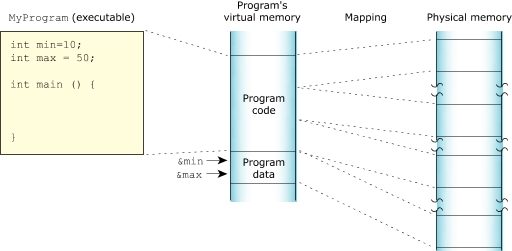
\includegraphics[width=9cm]{2.jpg}
		\caption{Program Memory}
	\end{figure}
\end{frame}

\begin{frame}{What the Stack memory looks like}
	\begin{figure}[h!]
		\centering
		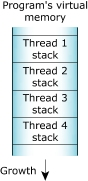
\includegraphics[width=3cm]{3.jpg}
		\caption{Stack Memory}
	\end{figure}
\end{frame}


\begin{frame}{What the Shared Libraries memory looks like}
	\begin{figure}[h!]
		\centering
		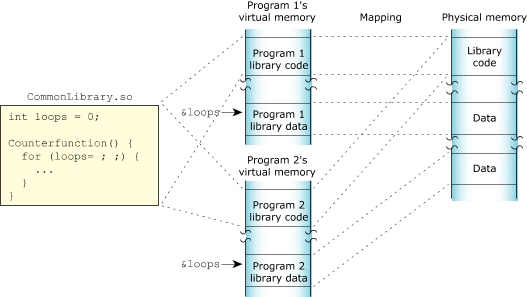
\includegraphics[width=9cm]{5.jpg}
		\caption{Libraries Memory}
	\end{figure}
\end{frame}

\begin{frame}{What the Objects memory looks like}
	\begin{figure}[h!]
		\centering
		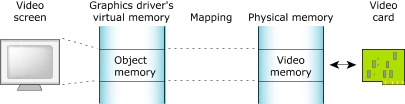
\includegraphics[width=9cm]{6.jpg}
		\caption{Objects Memory}
	\end{figure}
\end{frame}

\begin{frame}{What the Heap looks like and how it works}
	\begin{figure}[h!]
		\centering
		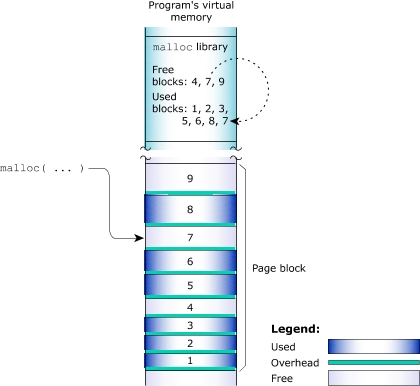
\includegraphics[width=6cm]{7.jpg}
		\caption{Heap Memory}
	\end{figure}
\end{frame}

\begin{frame}
	All images where taken from QNX Website at 
	\url{http://www.qnx.com}. \\
	\vspace{10pt}
	The User's Guide explain how memory works in QNX Neutrino IDE, but it's barelly the same everywhere.\\
	\vspace{10pt}
	Thank You for your attention.
\end{frame}

\end{document}